\chapter{使用工作区}\label{ch:workspace}
\chapterlead{工作区既是观察结构的地方，也是组织计算和保存结果的地方。本章从主窗口的各个区域入手，通过导入、查看、命名和保存一个硅结构项目，建立后续教程共同使用的操作习惯。}

\section{主窗口的布局}
\index{Gongzuoqu@工作区}
工作区把结构、计算步骤和结果放在同一个主窗口中。先认识初次进入时的空白布局，再展开练习中需要的面板，就容易分清“项目中有什么”和“当前正在编辑什么”。顶部功能区用于选择命令，中央文档区用于显示结构、工作流与图形；两侧面板提供项目条目、对象信息、计算参数和运行输出。

\subsection{初次进入工作区}
第一次进入空白项目时，中央显示欢迎文字，还没有打开结构或工作流文档。图\ref{fig:desktop-start}保留这一状态：左侧项目浏览器列出项目分类，信息浏览器位于左下方并折叠为标题栏，右侧面板组尚未展开。空白文档区是开始工作的地方；导入结构或建立工作流后，相应文档才会出现在这里。

\begin{figure}[!htb]
\centering
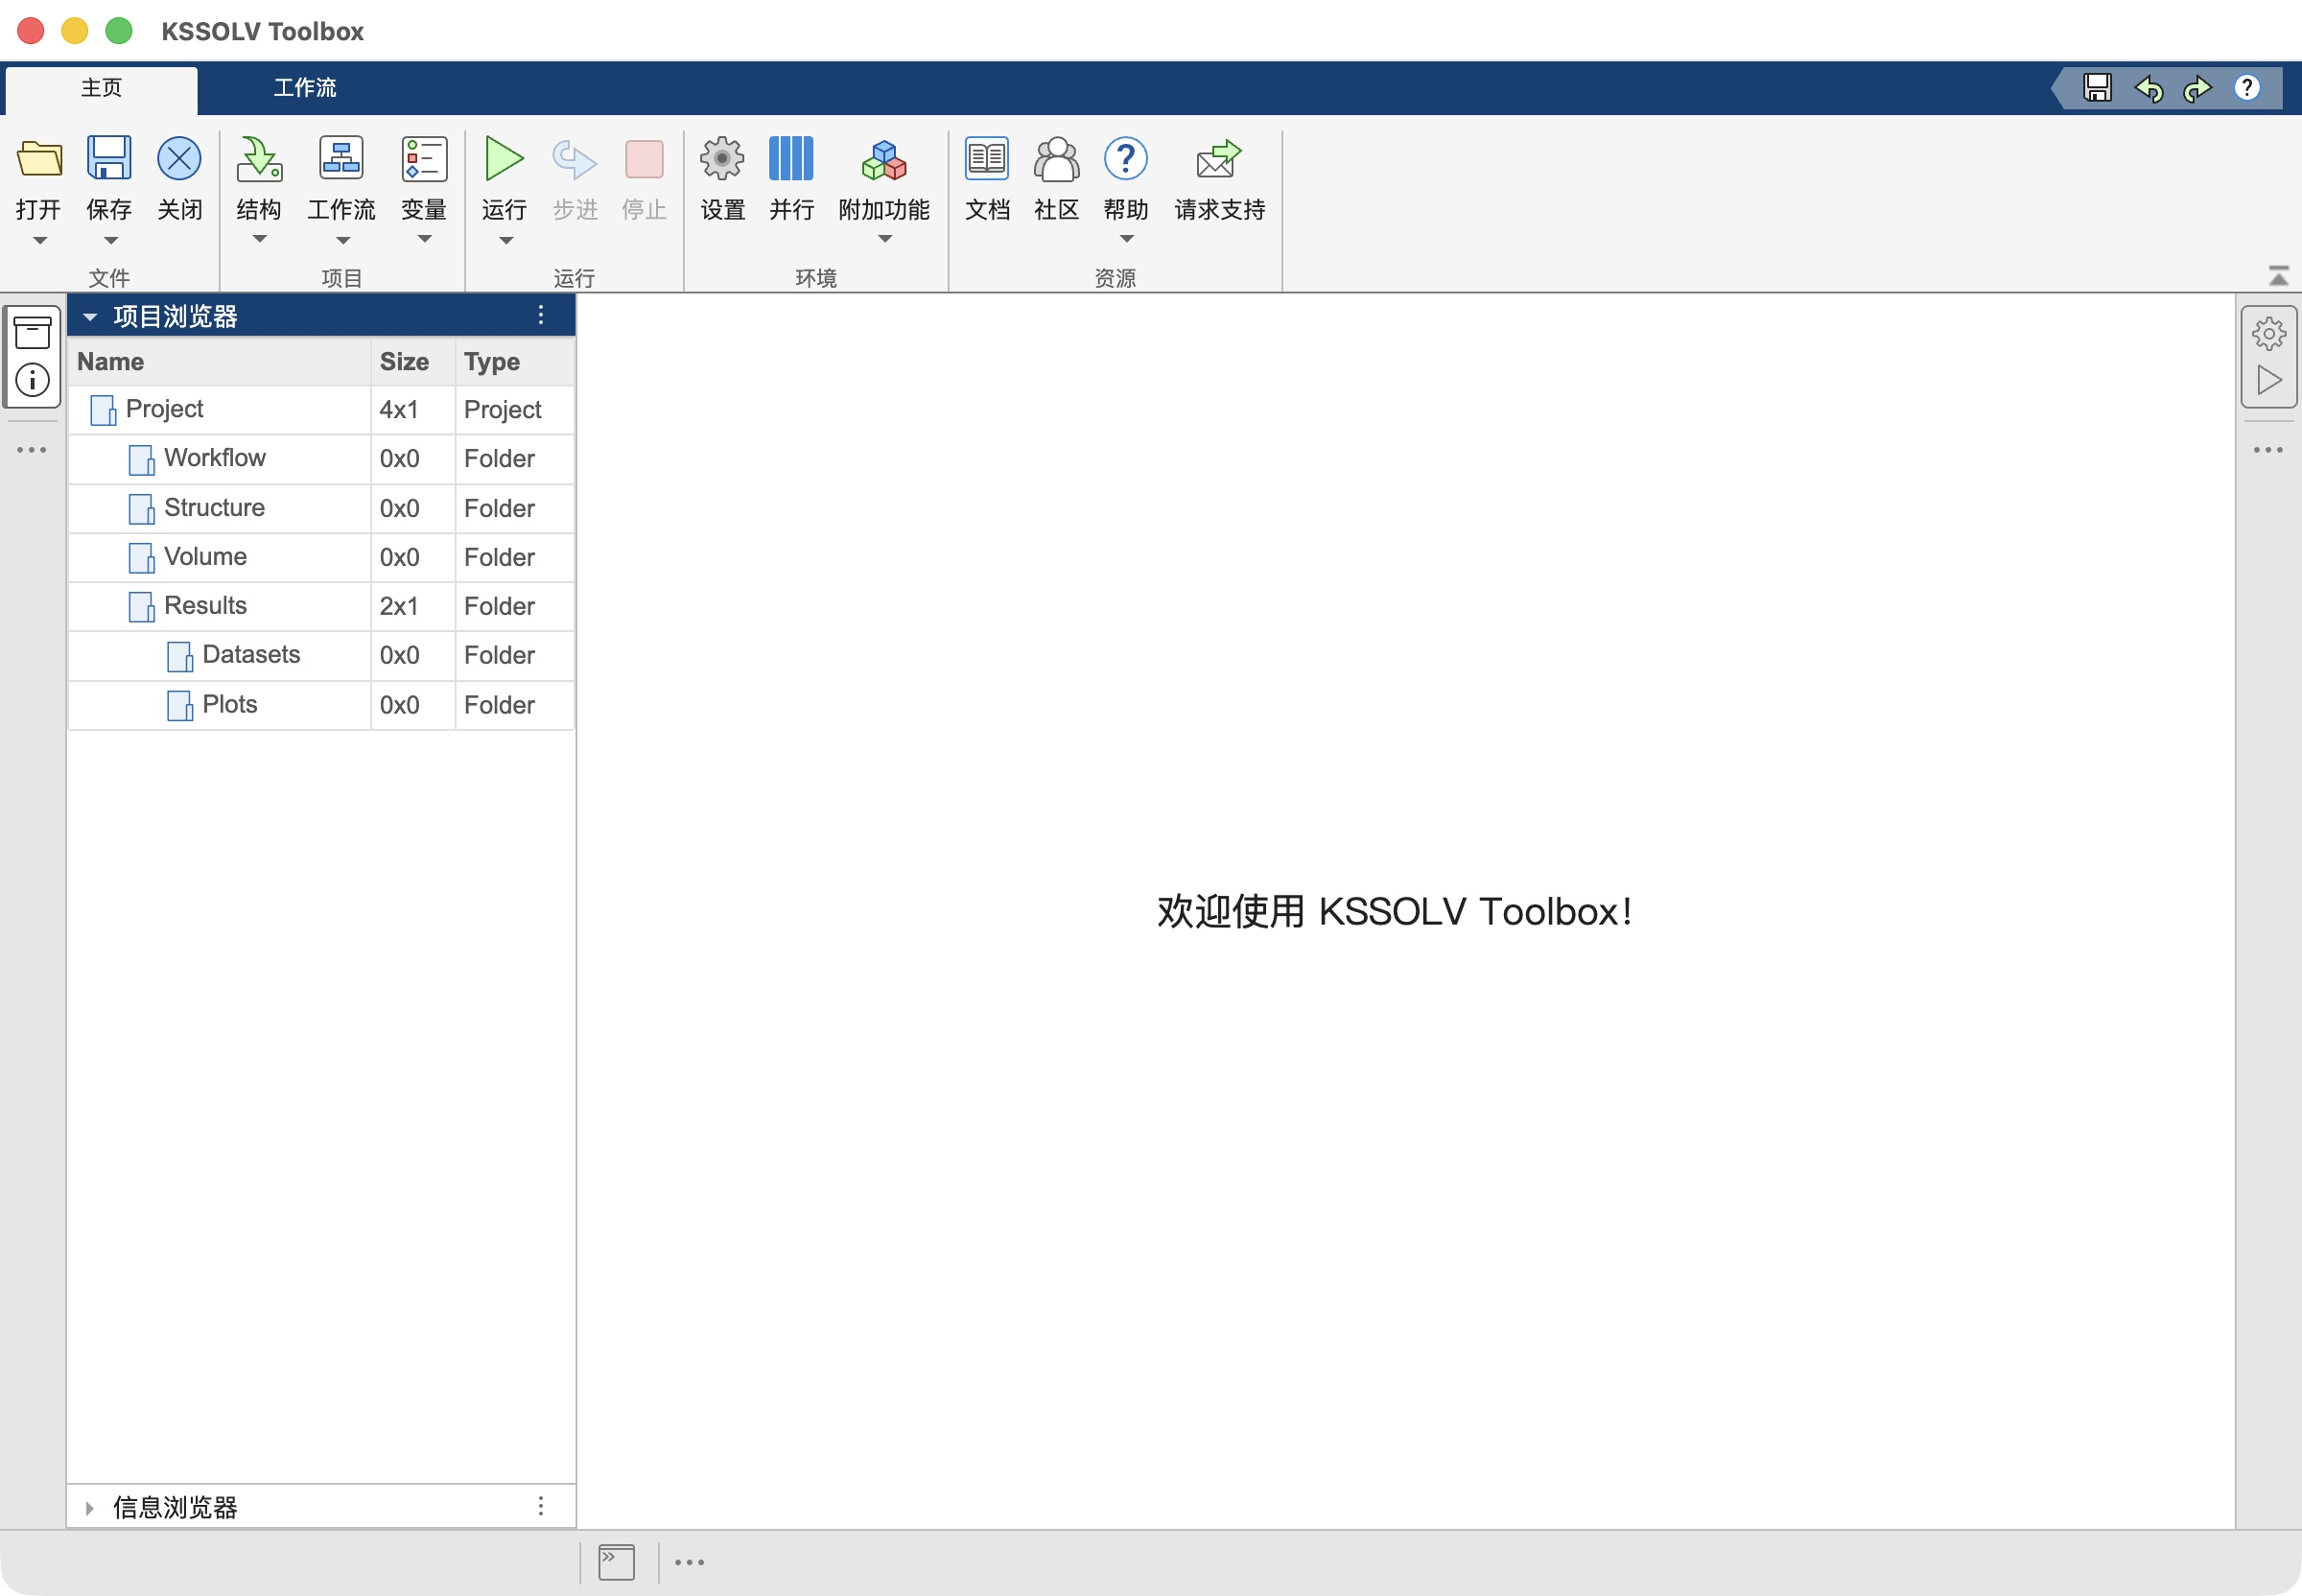
\includegraphics[width=\linewidth]{publication-assets/crop-eb25a0cdb09d3f78fdbd.png}
\caption{独立应用程序的初始工作区。中央尚未打开文档，左侧项目浏览器列出项目分类；信息浏览器折叠为标题栏，右侧面板组处于收起状态。}
\label{fig:desktop-start}
\end{figure}

可以先找到\ui{主页}中的\ui{结构}与\ui{工作流}入口，再观察窗口两侧的按钮。左侧的项目与信息图标控制同一组面板，右侧的配置与运行图标控制另一组面板；点击按钮组可以收起或展开这一侧的区域。组内面板标题前的小三角用于单独展开内容。需要的面板没有出现时，从侧边栏省略号打开\ui{打开面板}列表，按名称选择即可。

\subsection{展开练习需要的面板}
做第一次计算时，通常需要在项目、结构、工作流和参数之间来回查看。图\ref{fig:install-workspace-overview}仍是空项目，只为认识各区域而展开了面板：左侧显示项目与信息，右侧显示配置与模拟，下方打开命令行窗口，中央仍显示欢迎文字。这些面板是手动打开的，并非首次启动时全部显示。

可以依次展开左右面板组，打开各面板的内容，先熟悉它们的位置。导入结构或建立工作流后，项目树才会增加相应条目，中央也会出现文档标签。双击项目条目可以打开文档，再用标签选择当前活动文档：查看结构时，中央显示三维模型；切换到工作流标签时，中央显示节点和连线。准备配置节点或运行计算前，先核对活动标签中的工作流名称。



\begin{table}[!htb]
\centering
\caption{工作区的主要区域与第一次查看时的操作。}
\label{tab:workspace-regions}
\begin{tabularx}{\linewidth}{p{24mm}p{32mm}X}
\toprule
区域 & 在哪里 & 先做什么 \\
\midrule
功能区 & 窗口上方 & 在\ui{主页}找到结构导入、工作流、保存和运行入口。 \\
快捷工具条 & 窗口右上方 & 辨认保存、撤销、重做和帮助按钮。 \\
项目与信息面板 & 左侧按钮组内 & 辨认项目分类；导入结构后选择条目，查看它的信息。 \\
配置与模拟面板 & 右侧按钮组内 & 找到参数与输出区域；建立工作流后，再选择节点进行配置。 \\
文档区 & 窗口中央 & 空项目显示欢迎文字；打开文档后，用标签切换结构或工作流。 \\
命令行窗口 & 展开后的下方区域 & 需要交互命令时再使用；图形教程可先保留此面板或折叠它。 \\
分隔线与状态栏 & 面板边界及窗口底部 & 拖动分隔线调整空间；执行操作时留意底部状态文字。 \\
\bottomrule
\end{tabularx}
\end{table}

布局可以随任务调整。观察三维结构时，收起暂时不用的侧面板；填写计算参数时，给配置编辑器更多宽度。拖动面板边界可以改变左右宽度或上下比例，结构和工作流仍保留在项目中。后面各小节分别说明这些区域怎样使用；本章的硅晶体练习会从导入结构开始，逐步用到它们。

\subsection{功能区}
\ui{主页}包含文件、项目、运行、环境和资源等常用操作。\ui{打开}读取已有项目；\ui{保存}把当前工作写入项目文件；\ui{结构}菜单用于新建或导入结构；\ui{工作流}菜单提供创建、模板、导入与导出入口。执行计算时使用\ui{运行}，应用设置和帮助也从主页进入。

\ui{工作流}页面提供节点与画布操作。它与中央的工作流文档配合使用：先激活目标工作流，再添加、连接和配置节点。只有顶部切换到工作流页面，还不足以确定要执行哪个工作流，应同时查看中央文档标签。

当三维结构文档处于活动状态时，功能区会出现\ui{晶体建模}或\ui{分子建模}页面。它们是围绕当前文档提供的工具。切换到其他类型文档后，上下文页面可能随之变化。需要建模命令却看不到相应页面时，先回到结构标签，而不是重新导入结构。

\subsection{项目浏览器}
\index{Xiangmu liulanqi@项目浏览器}
项目浏览器以树形方式显示内容，主要分支为 \ui{Workflow}、\ui{Structure}、\ui{Volume} 和 \ui{Results}。结果下又可见 \ui{Datasets} 和 \ui{Plots}。这里的英文名称与界面一致，分别表示工作流、原子结构、体数据、数值数据和图形。

单击条目用于选择，双击可以打开相应文档。展开分支后，可同时保留多个项目项；关闭中央文档标签，只是结束这一个视图，不等于从项目中删除它。再次在树中双击，便可重新打开。选择删除操作则会改变项目内容，二者应分清。

树中的 \ui{Name} 是显示名称，\ui{Type} 表示对象类型。\ui{Size} 是项目项组织或数据尺寸信息，不宜直接当作体系原子数。判断一个晶体含多少独立原子，应查看结构信息或三维视图中的位点数。屏幕还可能显示相邻晶胞的映像，因此肉眼数到的球体也未必等于模型位点数。

\subsection{信息浏览器}
信息浏览器随项目浏览器的选择变化。选择一个结构时，可查看与该结构有关的属性；选择工作流、数据或图形时，面板显示对应对象的信息。它可以帮助确认当前处理的是哪一个条目，避免在相似文件名之间混淆。

部分条目允许编辑显示名称。修改后，应在项目树与文档标签中核对新名称。为结构命名时，写出材料和主要变化通常比 \file{Structure1} 更有用，例如 \file{Si-primitive}、\file{Si-2x2x2}、\file{Si-vacancy}。名称用于识别，不能代替实际检查晶胞和原子数。

\subsection{配置编辑器}
\index{Peizhi bianjiqi@配置编辑器}
配置编辑器用于修改工作流节点的参数。先在画布中选中节点，再点击\ui{工作流 → 配置节点}，或使用节点上的齿轮按钮。随后在右侧编辑器中向下查看该节点的\ui{选项}。节点名称、输入和输出等通用字段，与截断能、迭代次数等任务参数位于不同区域；只看到通用字段时，应先执行配置节点命令，再滚动查看选项。填写后切换到其他节点，再返回确认数值仍在，是检查输入是否提交的简便方法。

\subsection{查看运行输出}

\ui{模拟浏览器}显示运行输出。自洽场迭代、计算消息和错误信息往往从这里开始阅读。计算结束后，不要只看运行按钮是否恢复，还应检查输出末尾的结束消息，以及项目结果分支中新生成的数据。第\ref{ch:first}章将用一次小型计算说明如何判断完成状态。

\subsection{安排面板布局}
\index{Cebianlan@侧边栏}
文档区可以同时打开结构、工作流和图形标签。选择标签会改变当前活动文档。标签暂未显示时，将鼠标移到文档区上方，可查看文档标题与标签。运行工作流前，尤其要看清活动的工作流名称。多个相似任务并存时，给它们清楚命名，可以减少误运行。

主窗口两侧设有侧边栏按钮组。左侧的项目与信息图标属于同一组，右侧的配置与运行图标属于另一组。按钮组控制这一侧面板区域的收放：例如，收起左侧组时，项目浏览器与信息浏览器一起隐藏；重新展开后，可以继续使用这两个面板。右侧组展开后，可以同时查看配置编辑器与模拟浏览器。图\ref{fig:desktop-start}中的右侧组处于收起状态；图\ref{fig:install-workspace-overview}则展示手动展开后的布局。

组内各面板还可以单独折叠。初始工作区左下方的\ui{信息浏览器}只显示标题栏；点击标题前的小三角，可以展开下方的信息区。需要增加三维视图空间时，可以折叠某一面板，也可以收起整个侧边组，二者作用的范围不同。

侧边栏底部的省略号打开\ui{打开面板}列表。找不到某个面板时，按名称选择\ui{项目浏览器}、\ui{信息浏览器}、\ui{配置编辑器}、\ui{模拟浏览器}或\ui{命令行窗口}。图\ref{fig:panels-gallery}显示在线版中的同组入口，其中还提供\ui{文件}，用于管理云端目录；前述五个面板在独立版中也可打开。

\begin{figure}[!htb]
\centering
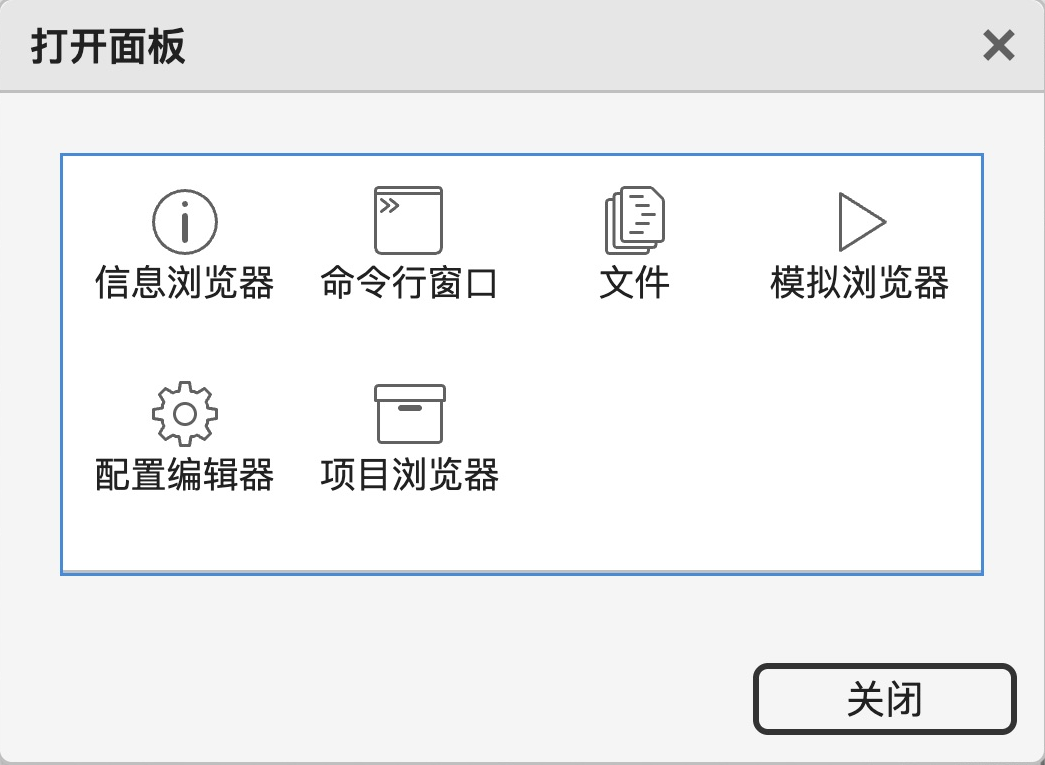
\includegraphics[width=88mm]{publication-assets/crop-50f2208998010f44014c.png}
\caption{实际打开的面板列表。这里按名称打开具体面板；两侧的按钮组则用于收放成组的面板区域。\ui{文件}用于管理云端目录。}
\label{fig:panels-gallery}
\end{figure}

观察三维模型时，可以收起暂时不用的参数和输出面板；编辑参数时，再展开配置编辑器。拖动文档区与面板之间的分隔线，可调整各区域宽度。同组面板之间的分隔线可调整上下比例。不同屏幕尺寸下，面板宽度可以有所不同，不必使布局与书中截图完全相同。

\section{练习：导入并检查硅晶体}
本例使用随书的 \file{silicon.cif}。它是边长约 $5.44370\,\text{\AA}$ 的硅常规晶胞，显式列出 8 个硅位点。文件采用 P1 方式列出所有位置，便于练习时直接核对原子数。该晶格常数是本例输入，不是这一步导入操作计算出的结果。

\begin{figure}[!htb]
\centering
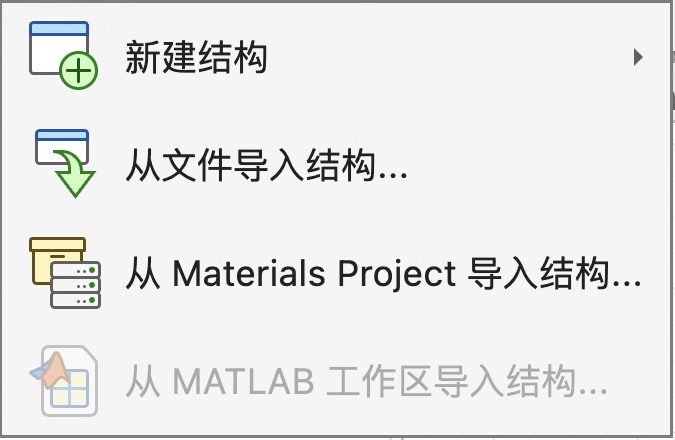
\includegraphics[width=67mm]{publication-assets/crop-e572efea8aa253089edc.png}
\caption{主页中的结构菜单。本练习选择\ui{从文件导入结构}；Materials Project 是另一个结构来源。\ui{从 MATLAB\regmark{} 工作区导入结构}需要 MATLAB\regmark{} 工具箱环境。}
\label{fig:structure-import-menu}
\end{figure}

\begin{steps}
\item 在\ui{主页}打开\ui{结构}菜单，选择\ui{从文件导入结构}。
\item 进入随书示例目录，选择 \file{silicon.cif}，确认打开。
\item 等待项目浏览器的 \ui{Structure} 分支出现 \file{silicon}，中央打开三维结构文档。
\item 拖动视图旋转，使用滚轮缩放。使整个晶胞位于画面中，不必立即调整所有显示参数。
\item 检查元素为 Si，模型独立位点为 8。若看到更多球体，查看它们是否属于边界或相邻晶胞的显示映像。
\item 单击一个位点，查看原子信息；使用空白处或相应选择命令清除选择，再观察完整结构。
\end{steps}

\begin{figure}[!htb]
\centering
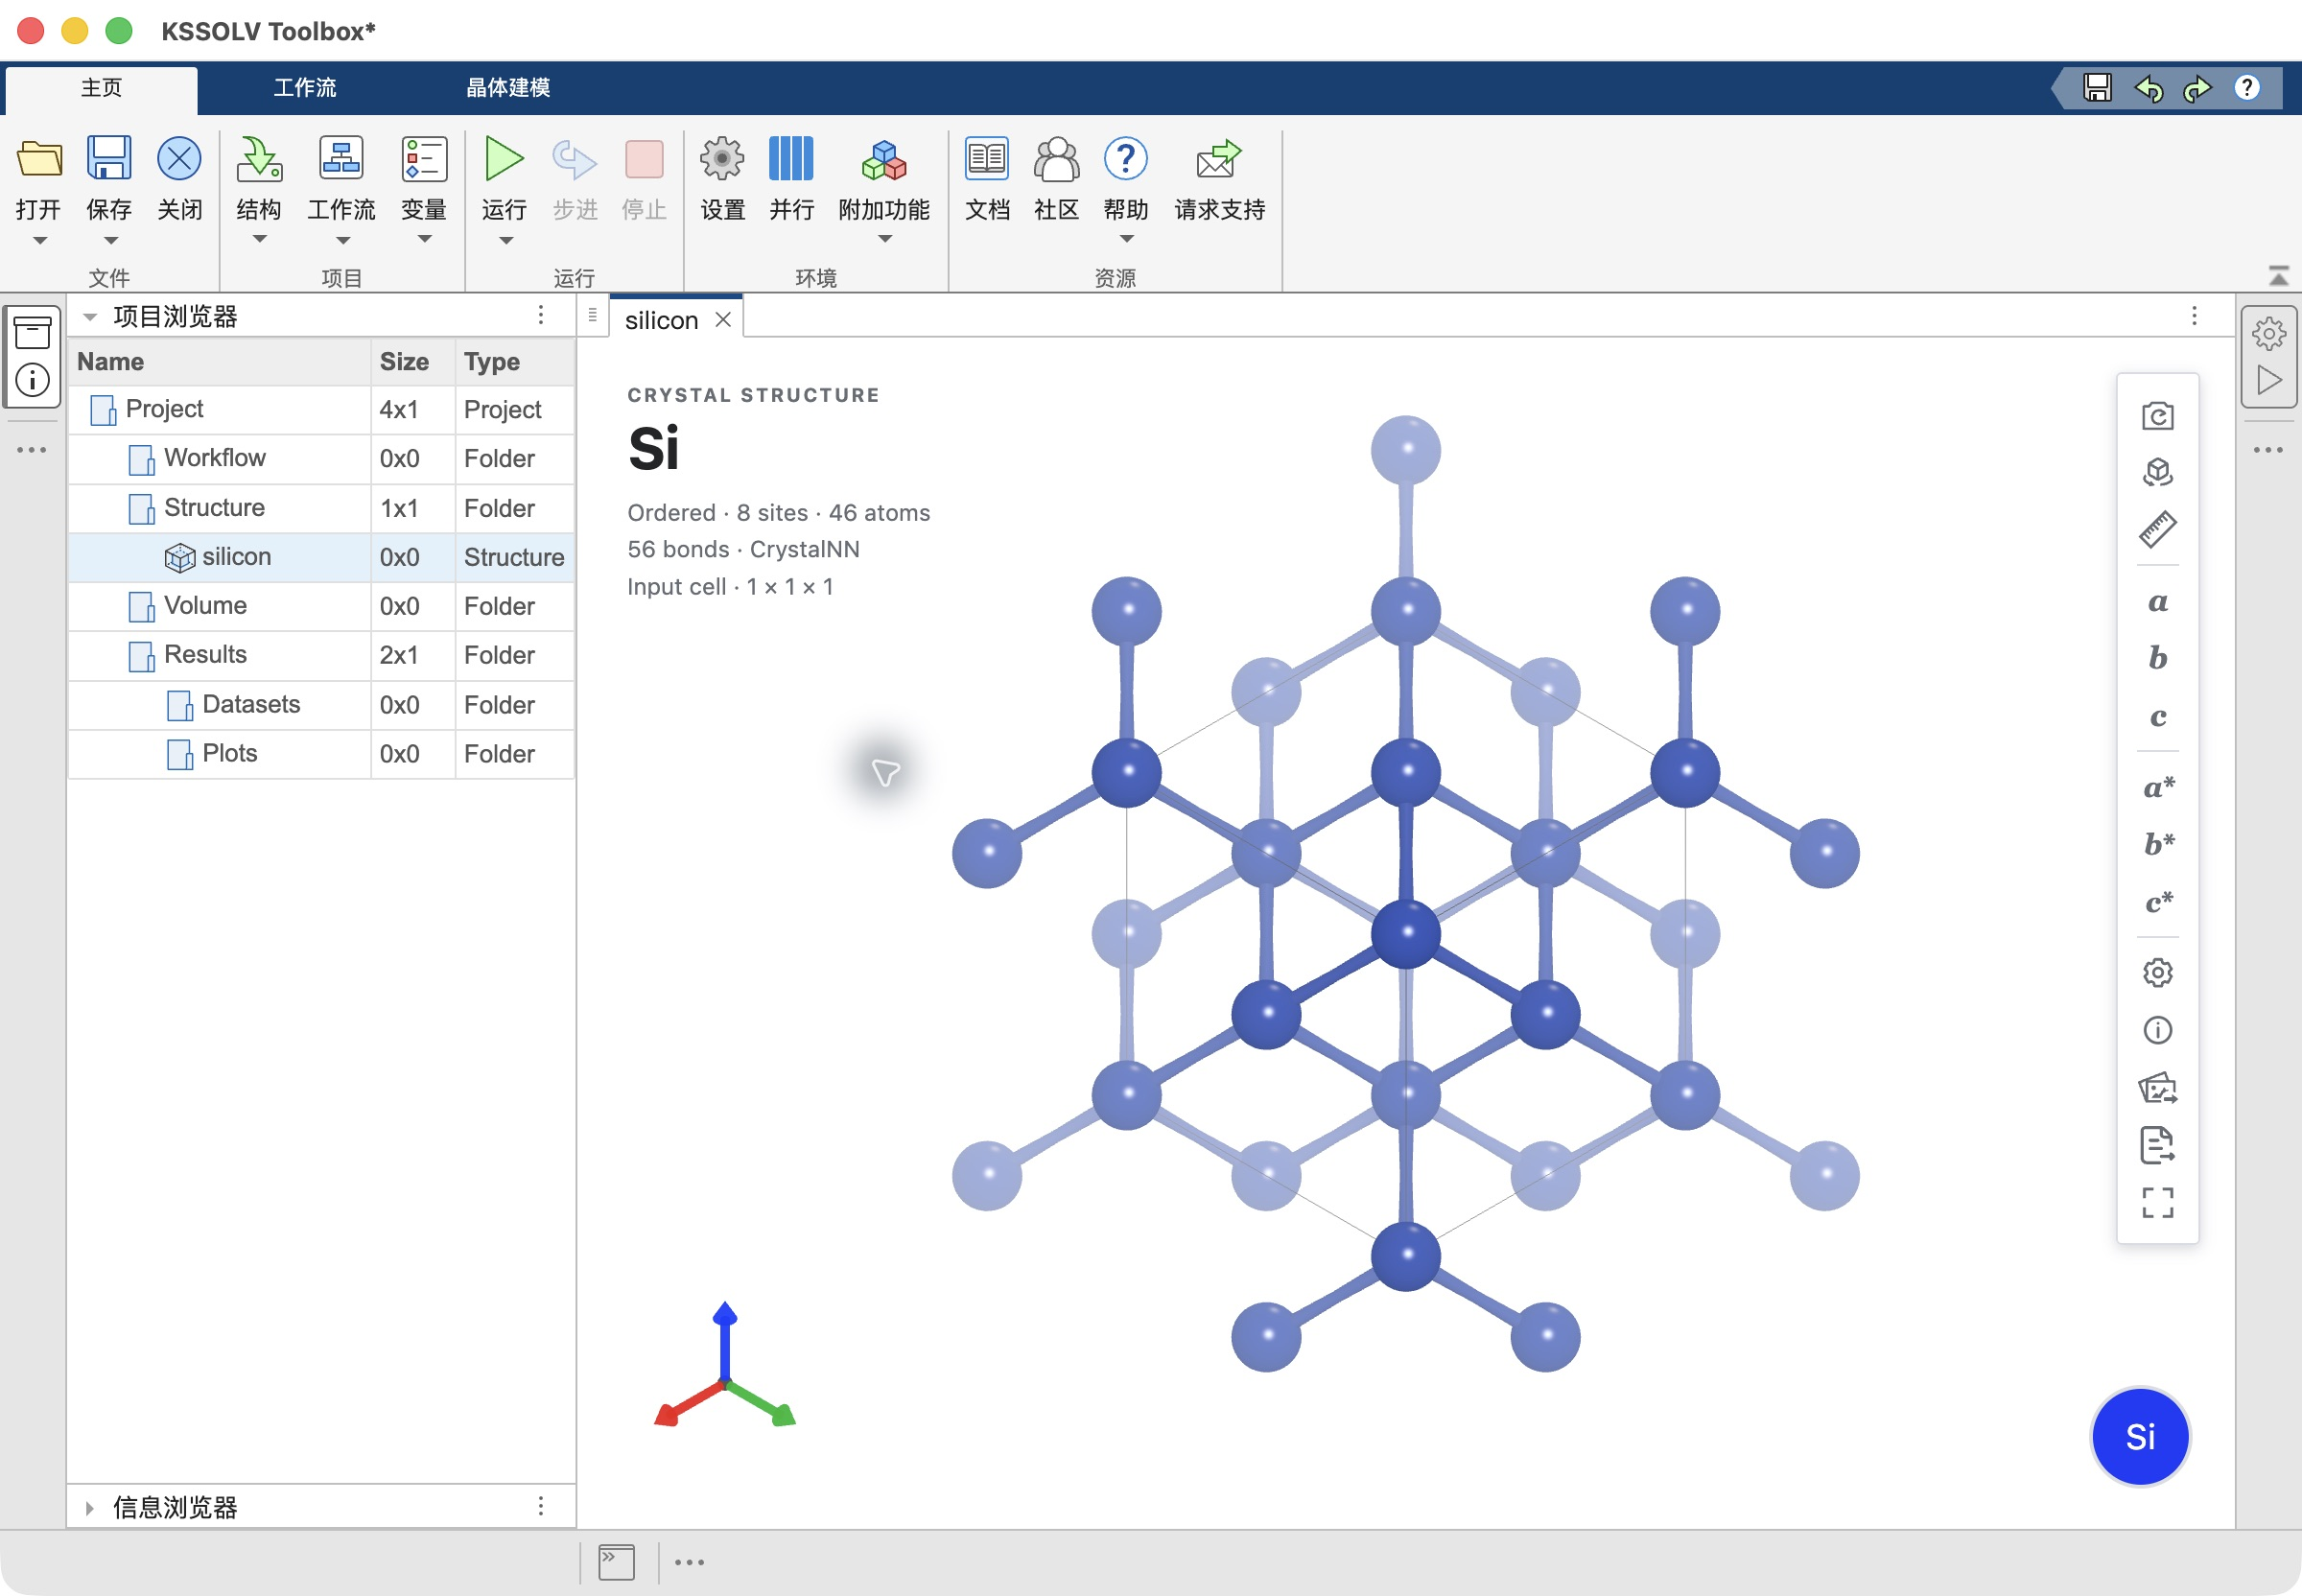
\includegraphics[width=\linewidth]{publication-assets/crop-693a9be4f512a9a0e125.png}
\caption{导入随书硅晶体后的结构文档。视图左上方显示\ui{8 sites · 46 atoms}：输入模型有 8 个位点，当前三维画面连同周期边界映像共绘制 46 个球体。}
\label{fig:silicon-import}
\end{figure}

\subsection{一次导入多个文件}

桌面文件选择器允许多选结构文件。需要比较一组模型时，使用\ui{从文件导入结构}，在文件窗口中选中这些输入后一起打开；每个成功读入的文件会成为独立的项目结构，而不是把所有原子自动拼成一个模型。

导入结束后，先在Structure分支核对实际增加的条目，再逐个打开检查。个别文件不能解析时，其他文件可能仍已导入，不能只凭打开过几个文件就假定项目中已有同样数量的可用模型。查看缺少的文件名与输出提示，单独处理该输入即可。在线版先将多个文件上传到云端目录，再按文件面板的导入方式逐项加入项目；上传成功本身不等于已经导入。


\subsection{读懂位点信息}
视图左上方概括当前结构和显示状态。本例的\ui{8 sites}对应文件列出的 8 个硅位点；\ui{46 atoms}表示当前画面中绘制的原子，包括周期边界附近的映像。下方的\ui{Input cell · 1 × 1 × 1}说明正在按输入晶胞显示。边界处显示更多球体，有助于看清跨晶胞的连接关系，并不表示输入已扩成含 46 个独立原子的模型。

在三维视图中选择一条硅—硅键，可以查看它连接的位点与几何长度。图\ref{fig:silicon-bond-inspection}的检查卡片显示\ui{Sites 2–7}，键长为 $2.35719\,\text{\AA}$，周期映像编号为\ui{0, 0, 0}。其中，位点编号用于对应模型中的原子；映像编号表示这条连接所用的晶胞平移。检查其他连接时，应同时看这两项。

\begin{figure}[!htb]
\centering
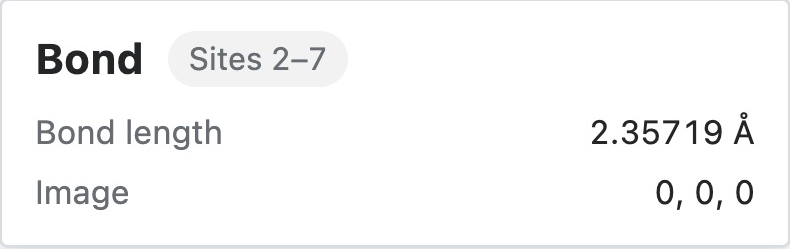
\includegraphics[width=79mm]{publication-assets/crop-6bd0b3f7b04c691f91a8.png}
\caption{选择硅—硅键后的检查卡局部。卡片中的 $2.35719\,\text{\AA}$ 来自本例输入结构的几何距离；此时尚未执行结构优化或电子结构计算。}
\label{fig:silicon-bond-inspection}
\end{figure}

完成检查后，清除选择，恢复完整视图。当前步骤的目的，是确认文件、模型位点和显示映像之间的对应关系。后续进行扩胞或结构优化时，也沿用这一检查方法：先读结构信息，再检查所关心的原子与连接。

若读取的是其他来源 CIF，导入后应先核对晶胞、占位、元素及原子数。不同文件可能使用原胞、常规晶胞或部分占位，不能仅凭化学式相同就假定结构相同。先把文件本身的描述认清，再决定是否转换或扩胞。

\section{保存项目}
\index{Baocun xiangmu@保存项目}
\subsection{首次保存}
\begin{steps}
\item 在\ui{主页}点击\ui{保存}。
\item 独立版选择自己的工作目录，输入 \file{Si-introduction.ks}。在线版按第\ref{ch:online}章的方法选择云端目录。
\item 确认保存后，查看窗口标题和项目文件名。
\item 再做一个容易识别的小改动，例如更改结构的显示名称，观察标题中的星号。
\item 再次保存，确认项目写入完成。
\end{steps}

标题中的星号表示尚有修改。保存既用于保留工作流和结果，也会处理结构编辑中的待保存内容。建模有预览、应用与保存几个阶段：预览用来检查，应用确认这一次修改，保存才把当前工作写入项目文件。第\ref{ch:modeling}章会通过实际编辑说明这些阶段。

\subsection{为不同研究保留副本}
当一个项目将用于多个不同条件时，可使用\ui{另存为}建立分支。例如，先保存原始硅项目，再另存成 \file{Si-supercell.ks} 做扩胞。这样能够保留清楚的起点。只更改项目名称不会自动改变模型，仍应在结构信息中确认是否已执行所需操作。

对同一个体系比较不同截断能时，也可在项目中保留多个明确命名的工作流。若结果较多或差异很大，分成多个项目更容易整理。选择哪种方式取决于工作习惯，关键是能从结果追溯到所用结构和参数。

\subsection{重新打开检查}
完成本例后，可关闭当前项目，再用\ui{打开}读取刚保存的 \file{.ks} 文件。展开结构分支，双击硅结构，检查它能重新显示。这个小练习确认保存的是可继续工作的项目，而不仅是当前屏幕上的一张图。

在线版中，重新打开云端项目与打开本机下载副本是两种入口。前者在文件面板选择已有 \file{.ks}；后者先上传本机副本。项目内容可以相同，存放位置仍需自己确认。

\subsection{关闭当前项目}

\ui{主页 → 关闭}关闭的是当前整份项目，不只是中央的一张结构标签。存在未保存的项目或结构编辑时，会询问保存、不保存或取消。希望继续留在原项目就选择\ui{取消}；选择保存后，应等待保存完成再进入空项目。关闭中央文档标签则保留项目树中的条目，需要时仍可再次打开。

\subsection{移除试算条目}

不再需要的工作流、结构或图形可以从项目中移除。先给准备保留的阶段另存副本，再选择确实不用的条目；不要用删除来代替关闭文档。

\begin{steps}
\item 在项目浏览器中单击一条试算记录，确认选择的是具体项目项，而不是Project或分类文件夹。
\item 让焦点留在项目树，按Backspace移除该项。删除当前工作流也可先选中其项目条目，再使用工作流页面的\ui{删除}。
\item 如果相应文档有未保存修改，按弹出的关闭提示选择；取消关闭时应回到项目树重新核对。
\item 检查留下的结构和流程仍然对应，再保存项目。删除项目项不等于删除最初从磁盘导入的源文件。
\end{steps}


\section{选择要保存的文件}
\index{Xiangmu wenjian@项目文件}
\file{.ks} 保存项目整体；\file{.wf} 保存工作流；CIF、POSCAR、XYZ 等文件主要保存结构。分享项目或练习结果时，应根据对方需要选择文件。希望对方接着计算，通常提供项目更方便；希望对方使用相同的任务组织方式，但更换材料，可以提供工作流模板；只交换几何结构，则导出相应结构文件。

结构文件能表达的内容与格式有关。CIF 适合晶胞和晶体位置，XYZ 直观地表达元素与笛卡尔坐标，但普通 XYZ 并不完整描述周期晶胞和显式化学键。保存重要的分子连接或复杂周期模型时，应查看所选格式能保留哪些内容，并在重新导入后检查。

\section{使用命令行窗口}
\index{Minglinghang@命令行窗口}
命令行窗口为需要交互命令的读者提供补充入口。独立应用和在线版中可使用发行包提供的函数与可用内置运算；本书的复算脚本在完整 MATLAB\regmark{} 中运行。常规导入、建模和工作流教程不要求使用命令行窗口。使用已有命令时，应先确认命令与当前工作区的对象对应，执行后再回到项目树或视图检查结果。

主页的\ui{文档}和\ui{帮助}提供进一步阅读；\ui{帮助 → 关于 KSSOLV}显示版本信息。遇到操作与书中不同时，先确认软件版本和当前文档类型；问题说明与日志整理见第~\ref{ch:troubleshooting}~章。

\subsection{执行一条简单命令}

从\ui{打开面板}列表打开\ui{命令行窗口}，将光标放在 \texttt{>>} 后的输入区。输入一条命令后按 Enter，输出会接在下方。下面的练习只使用简单数组，不改变项目结构。

\Needspace{5\baselineskip}
\begin{lstlisting}[language=Matlab]
a = [1 2 3];
sum(a)
\end{lstlisting}

逐行提交后，第二行应得到 6。输入\texttt{whos}可以查看当前命令工作空间中的变量。键盘上、下方向键用于回到已输入的命令；Tab 用于选择补全建议，Esc 关闭建议。输入\texttt{clc}清除窗口中的显示记录，但不等于删除变量。清空显示前，需要保留的命令与输出可以复制到自己的实验记录。

命令窗口的变量与项目树是两种保存方式。创建变量\texttt{a}不会在项目里自动增加一个结构，保存项目也不是保存命令窗口全部临时变量。希望保留结构、流程和结果时，回到项目树检查相应条目；希望重复执行一组命令时，在完整 MATLAB\regmark{} 中整理为脚本。

\section{使用快捷工具条}

主窗口上方的快捷工具条提供保存、撤销、重做和帮助。快捷保存与\ui{主页 → 保存}保存同一个项目，不是另存当前图片。窗口中同时打开多个文档时，先确认正在操作哪一个：结构文档活动时，撤销与重做针对该结构的建模历史；工作流文档活动时，针对流程图编辑。

\begin{steps}
\item 在三维结构中完成一次容易识别的编辑，观察修改后的状态。
\item 单击快捷工具条的\ui{撤销}，确认模型回到前一步；再单击\ui{重做}恢复。
\item 确认模型正确后，单击快捷\ui{保存}，核对项目的保存标记。
\end{steps}

完成第~\ref{ch:first}~章、建立第一条工作流后，还可以在画布中移动一个节点，再用撤销和重做比较两类编辑。

保存文件、执行计算和撤销编辑不是同一件事。撤销并不负责恢复外部文件或取消已经完成的科学计算；比较两次计算仍应保留不同结果和明确的参数说明。

\section{从 \headinglatin{Materials Project} 查找结构}\label{sec:mp-search}
\index{Materials Project@Materials Project!Jiansuo@检索结构}

数据库检索适合在尚无本地结构文件时寻找计算起点。先按第\ref{ch:remote}章在设置中保存自己的 Materials Project 访问密钥，再选择\ui{主页 → 结构 → 从 \mbox{Materials Project} 导入结构…}。检索窗口上方是查询条件，中间是元素周期表，下方是结果表与翻页按钮。导入后，可为选定结构继续建立计算工作流。

\subsection{选择检索方式}

\begin{table}[htbp]
\centering
\caption{Materials Project 的三种检索方式。}
\begin{tabularx}{\linewidth}{lX}
\toprule
方式 & 适用的查找问题 \\
\midrule
仅这些元素 & 在周期表选择元素，结果包含全部所选元素且不含其他元素；例如只选 Si，寻找单质硅。 \\
至少包含这些元素 & 所选元素必须出现，结果还可以有其他元素；例如先选 Fe、O，再查看含它们的材料。 \\
化学式 / MP ID & 直接输入化学式或已知材料标识；适合按已知记录查找。 \\
\bottomrule
\end{tabularx}
\end{table}

前两种方式由周期表按钮形成查询，顶部元素文本随选择更新；不要在不可编辑的元素框里输入化学式。想改用化学式时，先切换\ui{化学式 / MP ID}。\ui{清除元素}用于清掉周期表中已有的选择，便于开始新的元素组合。

\subsection{练习：查找一个硅结构}

\begin{steps}
\item 选择\ui{仅这些元素}，清除原有选择，再在周期表选择 Si。
\item 单击\ui{检索}，等待状态栏结束查询。若没有记录，先确认查询方式与元素选择，再检查访问设置。
\item 在结果中查看\ui{Material ID}、化学式、晶系、空间群和原子数。相同化学式可能对应不同结构，不能只凭第一行决定。
\item 每页条数可选10、15、20或30；用首尾页与前后页按钮继续查看。需要比较某列时，可单击表头排序当前结果。
\item 本例选择\ui{mp-149}，其晶系为Cubic、空间群为Fd-3m（227）、原子数为2。选择这一行，使\ui{导入所选结构}可用，单击导入并等待结构取得完成。
\item 关闭检索窗口，切回项目浏览器，找到新增加的 Structure 条目。打开三维文档，核对元素、晶胞和独立位点数，再保存项目。
\end{steps}

本次检索得到43条记录，数据库更新后数量和排列可能改变。mp-149导入的是两位点原胞，与八位点常规硅晶胞是同一晶体的不同晶胞表示；不能仅按原子数判断导入有误。数据库记录会更新，检索时按 Material ID 和结构信息确认材料。需要与随书硅数值逐项比较时，仍使用指定的\file{silicon.cif}或\file{silicon_primitive.cif}，保持输入一致。

结果表还显示体积、密度、带隙、形成能、凸包能和稳定性。单位已经写在列名中：带隙为 eV，形成能与凸包能为 eV/atom。这些数值来自数据库，引用时应注明相应记录。星号表示实验中已观测到的记录，不等于已经为当前任务完成精度检验。记录下 Material ID，有助于在报告中说明结构来源。


\begin{figure}[!htb]
\centering
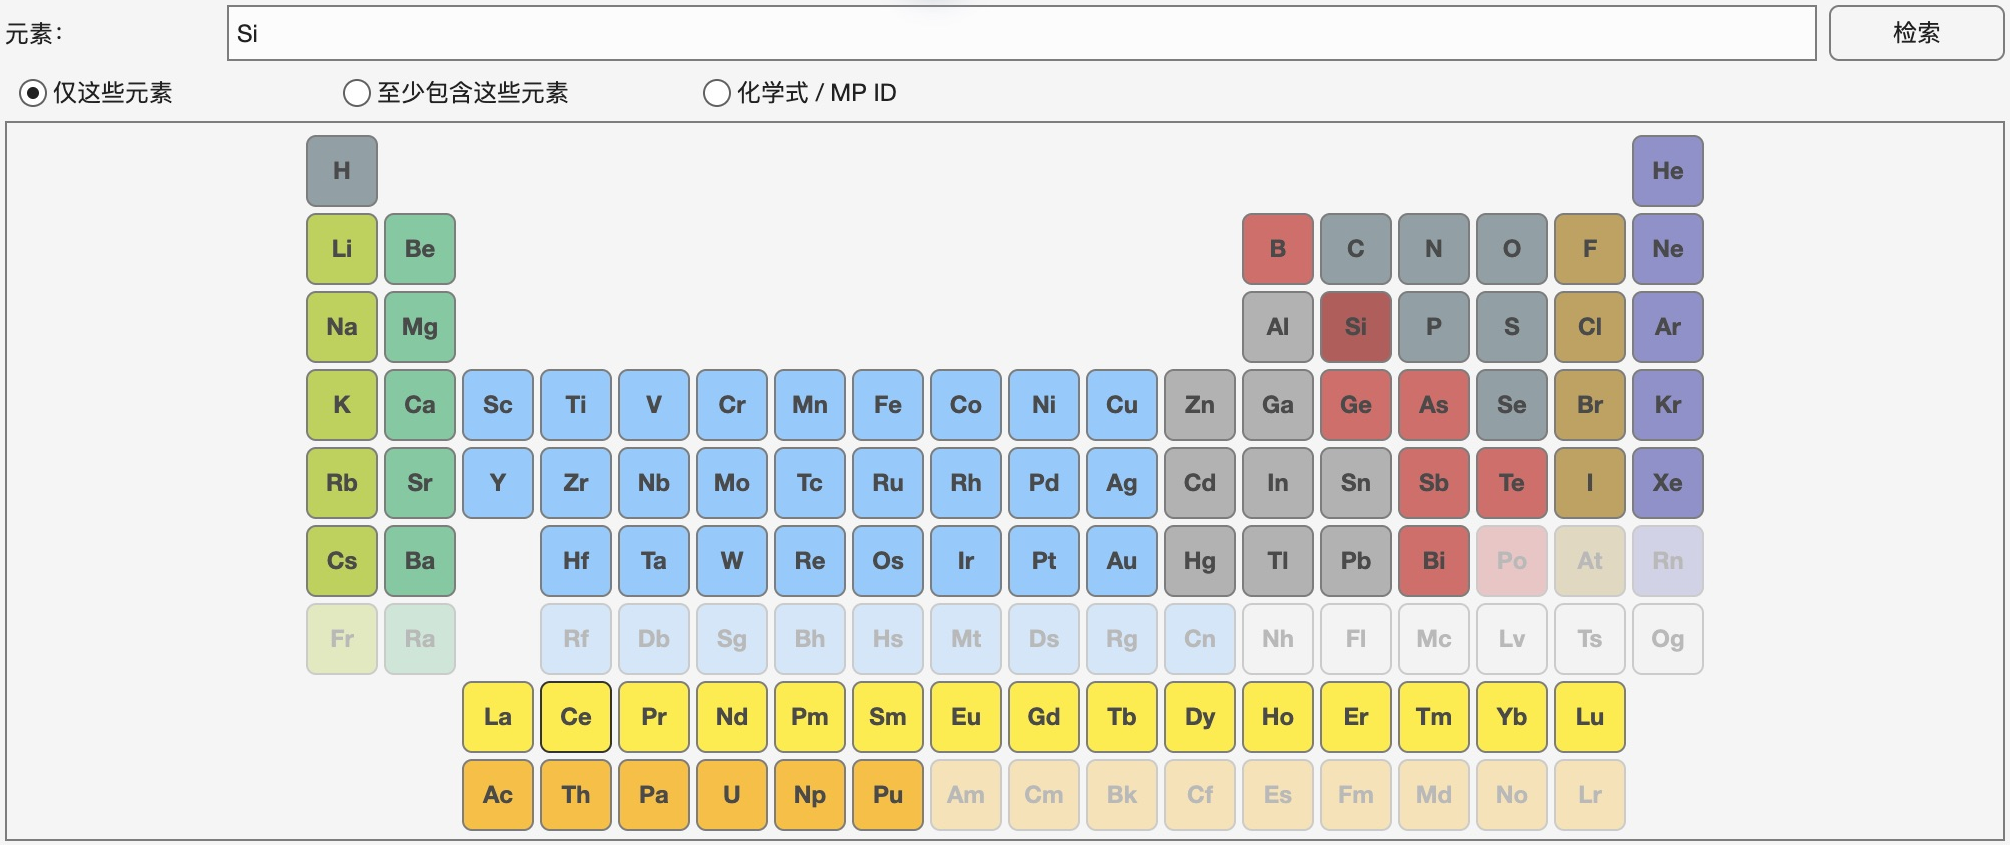
\includegraphics[width=\linewidth]{publication-assets/revision-materials-project-si-results.png}
\caption{在元素周期表选择Si，使用“仅这些元素”查找单质硅。查询方式与元素选择显示在结果表上方。}
\label{fig:mp-periodic-live}
\end{figure}

\begin{figure}[!htb]
\centering
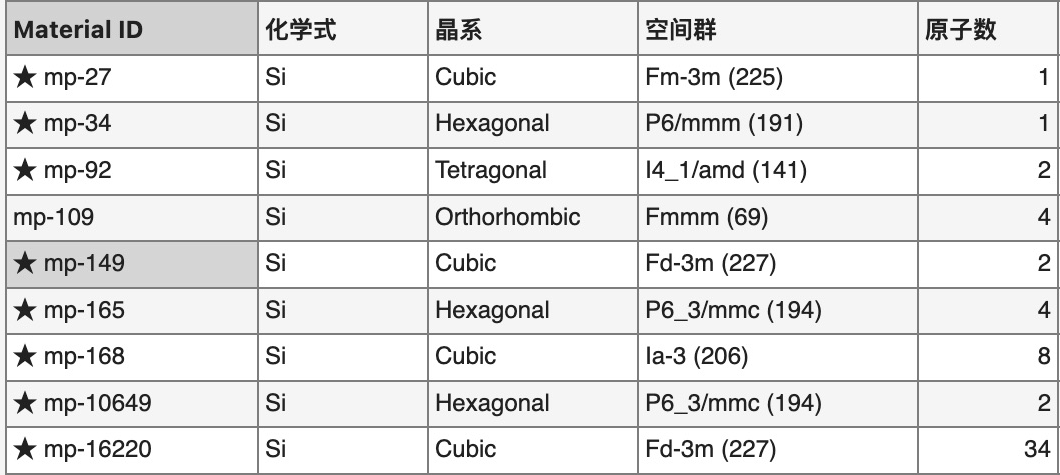
\includegraphics[width=\linewidth]{publication-assets/revision-materials-project-si-results-identity.png}
\caption{硅检索结果的标识列局部。此处选择mp-149：Cubic、Fd-3m（227）、两个原子；数据库中还有其他硅晶型。}
\label{fig:mp-results-live}
\end{figure}

\begin{figure}[!htb]
\centering
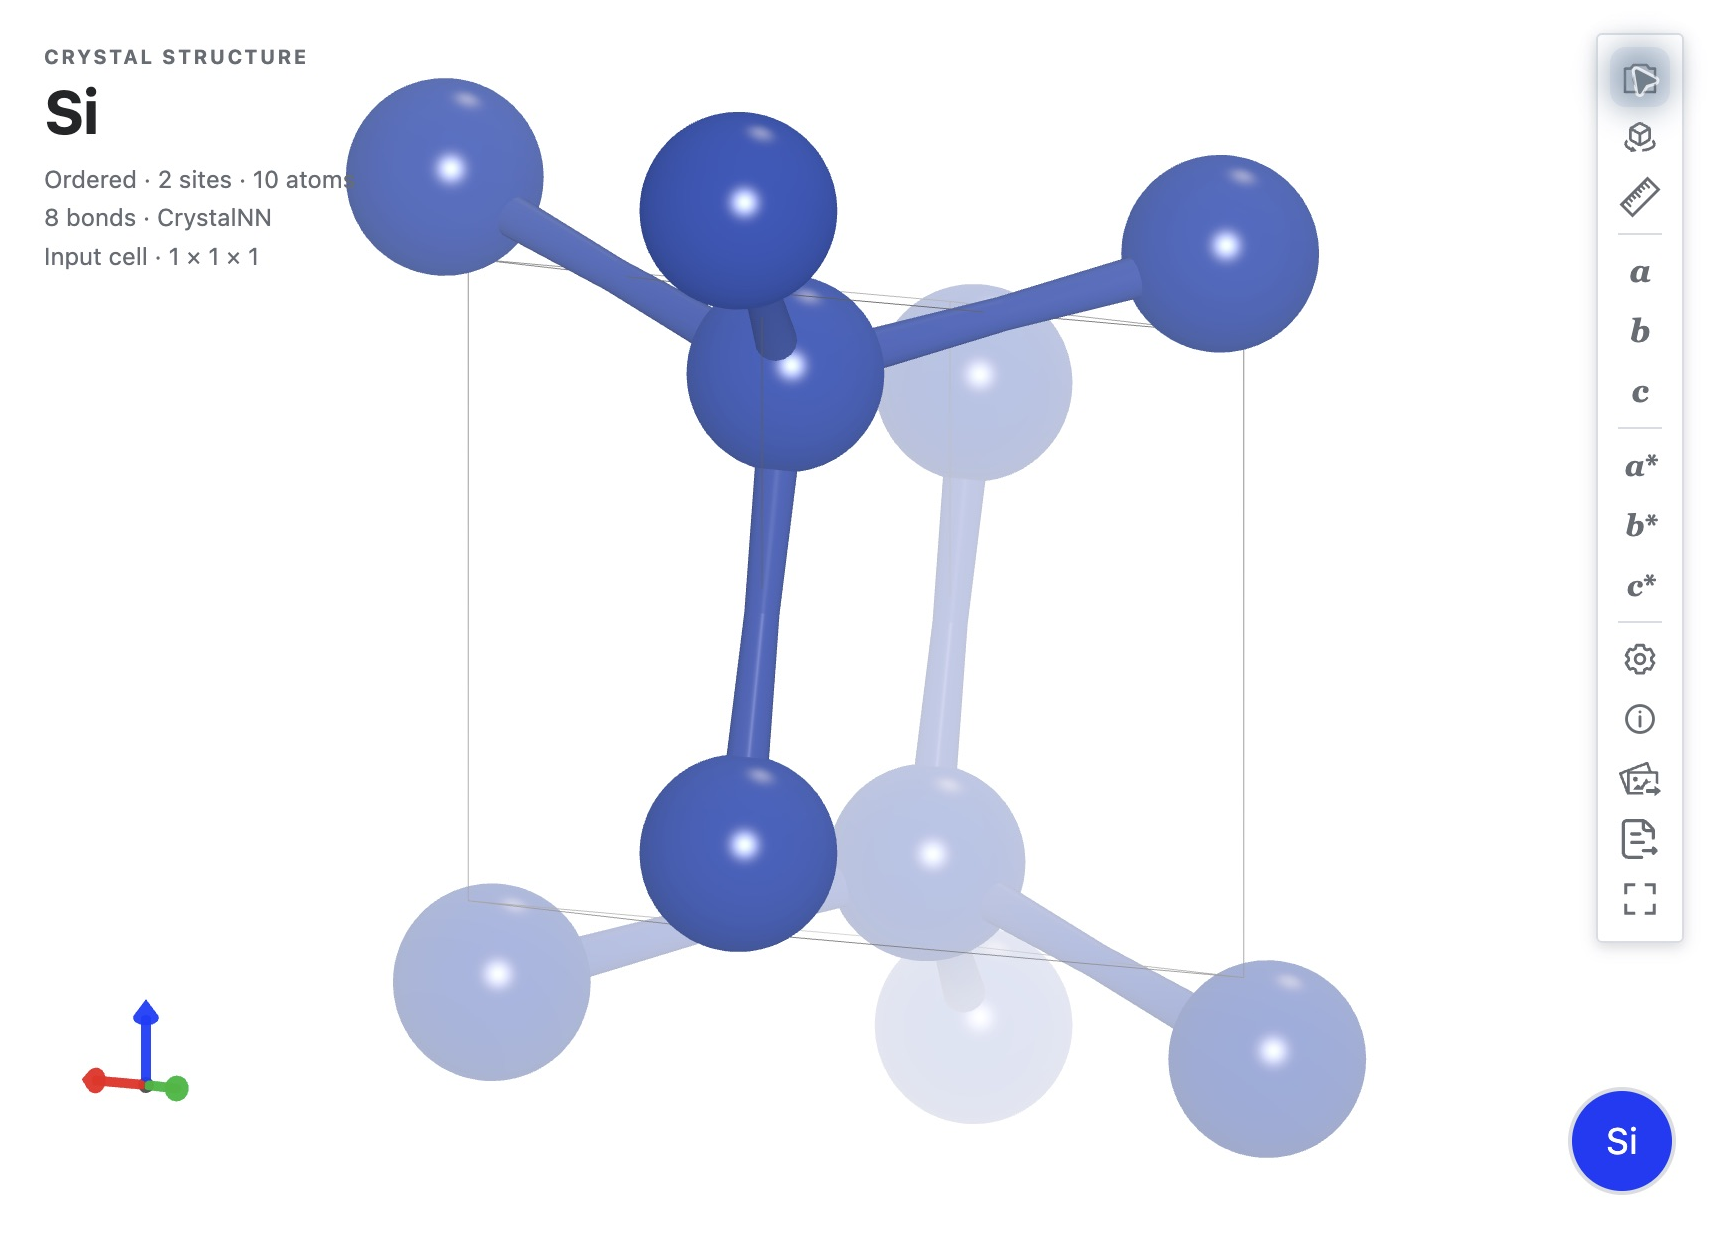
\includegraphics[width=\linewidth]{publication-assets/revision-materials-project-imported-si.png}
\caption{mp-149导入后自动打开的硅原胞视图。摘要显示两个独立位点，附加的半透明原子用于表示周期边界连接。}
\label{fig:mp-import-live}
\end{figure}



\section{完成本章后的检查}
现在应能在项目树中找到导入的硅结构，知道如何打开和关闭文档，能够收放侧边面板，并把工作保存为 \file{.ks} 项目。继续到第一项计算前，准备好随书的氢分子案例，保留当前硅项目。后续章节还会使用硅作为示例，进行数值比较时按各章指定的结构文件开始。
